\documentclass[12pt]{article}
% \usepackage[breaklinks=true]{hyperref}
% \usepackage[html,png]{tex4ht}
\usepackage{color}
\usepackage{amsmath,amssymb,amsthm}
\usepackage{natbib}
\usepackage{array}
\usepackage{booktabs, multicol, multirow}
\usepackage[nohead]{geometry}
\usepackage[singlespacing]{setspace}
\usepackage[bottom]{footmisc}
\usepackage{floatrow}
\usepackage{float}
\usepackage{caption}
\usepackage{indentfirst}
\usepackage{lscape}
\usepackage{floatrow}
\usepackage{epsfig}
\usepackage[usenames,dvipsnames,svgnames,table]{xcolor}
\usepackage[colorlinks=true,
            urlcolor=RawSienna,
            linkcolor=RawSienna,
            citecolor=NavyBlue]{hyperref}
\floatsetup[table]{capposition=top}
\floatsetup[figure]{capposition=top}


\newcommand{\beq}{\begin{equation}}
\newcommand{\eeq}{\end{equation}}

\newcommand{\cD}{{\mathcal D}}
\newcommand{\cF}{{\mathcal F}}
\newcommand{\todo}[1]{{\color{red}{TO DO: \sc #1}}}
\renewcommand{\baselinestretch}{1.5}

\title{Student Evaluations of Teaching (Mostly) Do Not Measure Teaching Effectiveness}
\author{Anne Boring, Kellie Ottoboni, Philip B.~Stark}
\date{Draft \today}
\begin{document}
\maketitle

\newpage
\begin{quotation}
    \emph{The truth will set you free, but first it will piss you off.}
    
     \hfill Gloria Steinem

\begin{abstract}

We examine whether student evaluations of teaching (SET) 
primarily measure teaching effectiveness, using nonparametric tests applied
to two datasets. 
Using the first dataset, 23,001~SET of 379~instructors by 4,423~students in six 
mandatory first year courses in a five-year natural experiment at a French university, 
we study relationships among SET and the genders of students and instructors, 
grade expectations, and grades.
Using the second dataset, 43~SET for 4~sections of an online course in a randomized, controlled, 
blind experiment at a US university, 
we study the relationships among SET, the genders of students, 
the actual and perceived genders of instructors, and grades.
On average, students rate apparently female instructors lower, by an amount that is large and
statistically significant.
On average, students who expect higher grades give higher ratings, 
by an amount that is statistically significant.
However, SET and apparent instructor gender are not significantly associated 
with an objective measure of teaching effectiveness,
student performance on anonymously graded finals. 
Evidently, SET are more sensitive to student biases and expectations than to teaching 
effectiveness.
There is strong statistical evidence that relying on SET for 
personnel decisions disadvantages female instructors.
The biases vary by student and by subject, making it 
difficult or impossible to adjust for the bias. 

% Nonparametric permutation tests that aggregate within 1,194 course sections show: 
%\begin{itemize}
%   \item the association between SET and final 
%            exam scores is negative but insignificant
%            ($P \approx 0.70$)
%   \item the association between SET and grade 
%            expectations is positive and highly significant
 %           ($P \approx 0.00$)
%   \item the association between instructor gender 
%            and final exam scores is insignificant
%            (students of male instructors do worse, $P\approx 0.51$ overall, $0.76$ for male students, $0.65$ for female students)
%   \item the association between instructor gender and SET is highly significant---because male
%             students rate male instructors higher 
%            (men get higher ratings, $P \approx 0.00$ overall, $0.00$ for male students,
%            $0.49$ for female students)
%\end{itemize}
%These relationships vary by discipline. 

%all first-year students take the same courses 
%(economics, history, political science, sociology, and %political institutions). 
%Students are assigned to sections of those courses as if %at random, creating a natural experiment.
%Final exams are set for the entire course
%by the professor rather than the section instructor, and %are graded anonymously.
%Hence, final exam scores are a proxy for the %effectiveness of the section instructors.
%SET are mandatory.
%
%Student responses fail simple tests of data quality.
%For instance, 29\% of students report spending impossible amounts of time
%on their courses.

\end{abstract}

\newpage

\end{quotation}

\section{Background}
Student evaluations of teaching (SET) are used widely 
in decisions about hiring, promoting, and firing instructors, especially non-tenured 
higher-education faculty. 
Universities generally treat SET as a measure of teaching effectiveness or teaching quality, 
rather than, e.g., a measure of student satisfaction.
Measuring teaching effectiveness is difficult---for students,
faculty, and administrators alike.
Evaluation surveys may measure something other than teaching effectiveness:
they may be consciously or unconsciously biased. 
In this article, we adopt the definition by \citet[p.17]{Centra2000}, according to whom 
biases in SET occur when ``a teacher
or course characteristic affects teacher evaluations, either positively or
negatively, but is unrelated to criteria of good teaching, such as increased student learning.'' 

Randomized experiments show that students confuse grades 
(or grade expectations) with long-term value \citep{Carrell2010a,Braga2014}. 
These experiments found that SET scores are not associated with 
student performance in follow-on courses, i.e., with teaching effectiveness. 
Instead, on average, high SET amount to a reward students give 
instructors who are easy graders or who ``teach to the test.''  

Gender matters too.
\citet{Boring2015} finds that SET are affected by gender biases and stereotypes. 
Male first-year undergraduate students tend to give more \textit{excellent} scores to male instructors,
even though there is no difference between
the academic performance of students of male and of female instructors.
Experimental work by \citet{MacNell2014} finds that
students rate the very same instructor lower on every aspect of teaching,
including putatively objective measures such as timeliness, when they think the instructor is 
female than when they think the instructor is male. 

Here, we use data from \citet{Boring2015} and \citet{MacNell2014} to investigate 
whether SET
primarily measure teaching effectiveness or something else: biases.
The two main sources of bias we study are students' grade expectations and the gender of the 
instructor. 
We also investigate variations in bias by discipline and by student gender.

We use permutation tests that allow us to avoid 
contrived, counterfactual assumptions about
parametric generative models for the data, which regression-based methods (including
ordinary linear regression, mixed effects models, logistic regression, etc.) and
methods such as $t$-tests and ANOVA generally require.
The null hypotheses for our tests are that some 
characteristic---e.g., instructor gender---amounts to an arbitrary label and might as well
have been assigned at random. 

We work with course-level summaries, matching how institutions use SET: 
typically, student responses in a course
are averaged, and those averages are compared across instances of the course,
across courses in a department, across instructors, and across departments.
\citet{StarkFreishtat2014} discuss statistical problems with this reduction to 
and reliance upon averages.

We find that associations between objective measures of teaching effectiveness and SET are weak
and not statistically significant.
Instructor gender is a stronger determinant of SET than teaching effectiveness is:
instructors perceived to be male receive significantly higher SET scores on average.
In the French data, \emph{male} students tend to rate male instructors higher
than they rate female instructors, with little difference in ratings by female students;
in the US data, \emph{female} students tend to rate (perceived) male instructors 
higher than they rate (perceived) female instructors, with little difference in ratings by male students. 
The French data also show that gender biases vary by course topic, and 
that students conflate grade expectations with teaching effectiveness.

We therefore conclude that SET primarily do not measure teaching effectiveness; that 
they are strongly and non-uniformly biased by factors such as the gender of the instructor
and student; and that it is impossible to adjust for these biases. 
SET should not be relied upon as a measure of teaching effectiveness.
Moreover, relying on SET for personnel decisions has disparate impact by gender. 

\section{Data}
\subsection{French Natural Experiment}
These data comprise a census of SET from first-year students at a French university.
The data, collected between 2008 and 2013, include 23,001 SET from
4,423 students (57\% women) in 1,177
sections, taught by 379 instructors (34\% women). 
The data are not public, owing to French restrictions on human subjects data.
\citet{Boring2015} describes the data in detail; key features include:
\begin{itemize}
   \item All first-year students take the same six mandatory courses: 
            History, Macroeconomics, Microeconomics, 
            Political Institutions, Political Science, and Sociology.
            Each course has one (male) professor
            who delivers the lectures, to groups of approximately 900 students. 
            Courses have sections of 10--24 students. 
            Those sections are taught by a variety of instructors, male and female.
            The instructors have considerable pedagogical freedom.
    
   \item Students enroll in ``triads'' of sections of these courses. 
            The enrollment process
            does not allow students to select individual instructors.
            The assignment of instructors to sets of students is ``as if'' at random,
            forming a \emph{natural experiment}.
            The assignment can be treated as if it is independent across 
            courses.
            
   \item Section instructors assign interim grades during the semester.
            Interim grades are known to the students before they submit SET.
            Interim grades hence create student grade expectations.
            
   \item Final exams are written by the professor, not the instructors.
            Students in all sections of a given course take the same final.
            Final exams are graded anonymously (except in Political
            Institutions, which we therefore omit from analyses involving final exam scores).
            Performance on the final exam is therefore a measure of the value the
            section instructor adds: students of more effective instructors should do better on
            the final exam, on average.
    
   \item SET are mandatory: response rates are nearly 100\%.
   
\end{itemize}

SET include closed- and open-ended questions.
The item that attracts the most attention is the \emph{overall score}, 
which is treated as a summary of the other items.

The SET data include students' individual evaluations of section
instructors in microeconomics, history, political institutions, and 
macroeconomics for the five academic years 2008--2013, and for 
sociology and political science for the three academic years 2010--2013 
(these two subjects were introduced in 2010). 
The SET are anonymous to the instructors, who have access to the ratings only after 
all grades have been officially recorded.  

\begin{table}[htbp]
  \centering
  \footnotesize 
  \caption{Summary statistics of sections}
    \begin{tabular}{lccc}
    \toprule 
    subject     & \# sections & \# instructors  & \% Female instructors  \\
   \midrule
  \textbf{Overall} &  \textbf{1,194} & \textbf{379}  &\textbf{33.8\%} \\
    History    &               230 &      72          &   30.6\% \\
    Political Institutions  &  229 &      65          &   20.0\% \\    
    Microeconomics   &         230 &      96          &   38.5\% \\
    Macroeconomics   &         230 &      93          &   34.4\% \\
    Political Science &       137 &      49          &   32.7\% \\
    Sociology   &              138 &      56          &   46.4\%    \\
    \bottomrule
    \end{tabular}%
 \label{tab:description}%
 
\textit{Data for a section of Political Institutions that 
had an experimental online format are omitted.
Political Science and Sociology originally were not in the triad system; 
students were randomly assigned by the administration to different sections.
} 

\end{table}%
\normalsize
Overall, 34\% of the 1,194 instruction sections were taught by women 
(Table~\ref{tab:description}), but the percentage varies by discipline. 
Only 20\% of Political Institutions sections were taught by women. 
Sociology is divided approximately equally between male and female instructors 
(46.4\% of sections were taught by women). 
Microeconomics and Macroeconomics have more instructors in all, because of higher turnover.

\subsection{U.S. Randomized Experiment}
These data, described in detail by \cite{MacNell2014}, are available online at 
\url{http://n2t.net/ark:/b6078/d1mw2k}.
Students in an online course were randomized into 6 sections of about a dozen students each, 
two taught by the primary professor,
two taught by a female graduate teaching assistant (TA), and two taught by a male TA.
In one of the two sections taught by each TA, the TA used her or his
true name; in the other, she or he used the other TA's identity.
Thus, in two sections, the students were led to believe they were being taught by a woman
and in two they were led to believe they were being taught by a man.
Students had no direct contact with TAs: the primary interactions were through
discussion boards.
The TA credentials presented to the students were comparable; the TAs covered
the same material; and assignments at the same time in all four sections taught by TAs.

SET included an overall score and questions relating to
professionalism, respectfulness, care, enthusiasm, communication, helpfulness,
feedback, promptness, consistency, fairness, responsiveness, praise, knowledge, 
and clarity.
Fourty-seven students in the four sections taught by TAs finished the class,
of whom 43 completed SET.
The SET data include the genders and birth years of the students; the grade data do not.
The SET data are not linked to the grade data.

\section{Methods and Notation} \label{sec:methods}

We use the Neyman ``potential outcomes'' framework.
A fixed number $N$ of individuals---e.g., students or classes---are assigned either
randomly or as if at random by Nature into 
$k \ge 2$ groups of sizes $N_1, \ldots, N_k$.
Each group receives a different treatment.
``Treatment'' is notional. 
For instance, the treatment might be the gender of the
class instructor.

For each individual $i$, we observe a numerical response $R_i$.
If individual $i$ is assigned to treatment $j$, then $R_i = r_{ij}$.
The numbers $\{r_{ij}\}$ are considered to have been fixed before the experiment.
Implicit in this notation is the \emph{non-interference} assumption that
each individual's response depends only on the treatment that individual receives, 
and not on which treatments other individuals receive.
We observe only one potential outcome for individual $i$, 
depending on which treatment she or he receives.
In this model, the responses $\{R_i\}_{i=1}^N$ are random, but only because individuals are 
assigned to treatments at random.

Our tests involve probability distributions induced by the random
assignment, with no assumption about the distribution of SET or other variables, 
no parameter estimates, and no models other than the potential outcomes 
framework.

\subsection{Illustration: French natural Experiment}
Consider the French data described above. 
The selection of course sections by students---and the implicit assignment of instructors to cohorts of students---is as if at random within 
disciplines, independent across disciplines.
However, the ``triad'' system keeps groups students together in their classes in different disciplines.
Hence, an appropriate hypothetical randomization would keep groups of students
together, and randomize the assignment of instructors across classes within
each discipline, independently across disciplines.

Consider testing whether, overall, SET are associated with final exam scores.
As the test statistic, we use the sum of the Pearson correlation coefficients between
average SET and average final exam score for sections of each subject; in principle,
positive correlations for some course subjects might offset negative correlations for others.
If SET do measure instructors' contributions to learning, we would expect this sum of
correlations to be positive: higher average SET in each discipline would tend to occur
in sections with high average final exam scores.

How surprising is the observed sum, if there is no (overall) connection between
average SET and average final exam for sections of a course?
The number $i$ of ``individuals'' is 950, the number of course sections of subjects other
than Political Institutions, because the final exam in Political Institutions is oral (and hence not
graded anonymously).
Each of the 950 course sections has an average SET and an average final exam score.
There were 224 sections of History, 229 of Macroeconomics, 226 of Microeconomics,
135 of Political Science, and 136 of Sociology. \todo{these numbers are from the ipynb, which
disagrees with the table \ref{tab:description} above. Why the discrepancy?}
Under the hypothetical randomization, within each of those five subjects, the instructors
were assigned sections as if at random, independently across subjects, with
the number of sections of each subject that each instructor teaches held fixed.
For instance, if there were $N_H$ sections of History taught by $K_H$ instructors in all,
with instructor $k$ teaching $N_{Hk}$ sections, then in the hypothetical randomization,
all
\beq
    {N_H}\choose{N_{H1} \cdots N_{HK_H}}
\eeq
assignments of the specified number of History sections to each History instructor 
would be equally likely.
The same would hold for sections of other courses,
and each combination of assignments across courses would be equally likely,
owing to the assumption that the assignments are independent.

Under the null hypothesis that SET have no connection to final exam scores,
final exam averages for sections in each course subject are exchangeable given the average SET
for the sections.
Imagine ``shuffling'' the average final exam scores across sections of each course, independently
for different courses.
For each shuffle, compute the Pearson correlation between average SET for each section
and average final exam score for each section, for each course subject.
Add the five Pearson correlations.
The distribution of this sum is the null distribution of the test statistic.
The $p$-value is the upper tail probability of that distribution beyond the observed value of the 
test statistic.
\todo{more here}

\subsection{Illustration: US Experiment}
As another illustration, consider the experiment conducted by \citet{MacNell2014},
in which $N$ students were assigned at random to six sections of an online course,
of which four were taught by TAs.
The analysis focuses on the four sections taught by TAs.
We condition on the assignment of students to the two sections taught by the professor.
Each remaining student $i$ could be assigned to any of $k=4$ treatment conditions:
either of two TAs, each identified as either male or female.
The assignment of students to sections was made at random: each of the
\beq
 {{N}\choose{N_1 N_2 N_3 N_4}} = \frac{N!}{N_1! N_2! N_3! N_4!}
\eeq
possible assignments of $N_1$ students to TA A identified as male,
$N_2$ student to TA A identified as female, etc., was equally likely.

Let $r_{i1}$ and $r_{i2}$ be the ratings student $i$ would give TA A when TA 
A is identified as male and as female, respectively; and let 
$r_{i3}$ and $r_{i4}$ the ratings student $i$ would give TA B when that TA
is identified as male and as female, respectively.
Typically, the null hypotheses we test assert that for each $i$, some subset of
$\{r_{ij}\}$ are  equal.
For assessing whether the identified gender of the TA affects SET,
the null hypothesis is that for each $i$,
$r_{i1} = r_{i2}$ (the rating the $i$th student would give TA A is the same,
whether TA A is identified as male or female), 
and $r_{i3} = r_{i4}$ (the rating the $i$th student would give TA B is
the same, whether TA B is identified as male or female).
Different students might give different ratings under the same treatment condition
(the null does not assert that $r_{ij} = r_{\ell j}$ for $i \ne \ell$), and
the $i$th student might 
give different ratings to TA A and TA B
(the null does not assert that $r_{i1} = r_{i3}$).
The null hypothesis makes no assertion about the population distributions of 
$\{r_{i1}\}$ and $\{r_{i3}\}$, nor does it assert that $\{r_{ij}\}$ are 
a sample from some super-population.

For student $i$, we observe exactly one of $\{r_{i1}, r_{i2}, r_{i3}, r_{i4}\}$.
If we observe $r_{i1}$, then---if the null hypothesis is true---we also know what $r_{i2}$ is,
and vice versa, but we do not know anything about $r_{i3}$ or $r_{i4}$.
Similarly, if we observe either $r_{i3}$ or $r_{i4}$ and the null hypothesis is true,
we know the value of both, but we do not know anything about $r_{i1}$ or $r_{i2}$.

Consider the average SET (for any particular item)
given by the $N_2 + N_4$ students
assigned to sections taught by an apparently female TA, minus the 
average SET given by the $N_1 + N_3$ students
assigned to sections taught by an apparently male TA.
This is what \cite{MacNell2014} tabulate as their key result.
If the perceived gender of the TA made no difference in how students rated 
the TA, we would expect the difference of averages to be close to
zero.\footnote{%
We would expect it to be a least a little different from zero both because of the luck of the draw
in assigning students to sections and because students might rate the two TAs
differently, regardless of the TA's perceived gender, and the groups are not all the same size.
}
How ``surprising'' is the observed difference in averages?

Consider the
\beq
{{N_1 + N_2} \choose {N_1}} \times {{N_3+N_4} \choose {N_3}}
\eeq
assignments that keep the same $N_1 + N_2$ students in TA A's
sections (but might change which of those sections a student is in) 
and the same $N_3 + N_4$ students in TA B's sections.
For each of those assignments, we know what $\{R_i\}_{i=1}^N$ would
have been if the null hypothesis is true: each would be exactly the same
as its observed value, since those
assignments keep students in sections taught by the same TA.
Hence, we can calculate the value that the test statistic would have had for each
of those assignments.

Because all ${N}\choose{N_1 N_2 N_3 N_4}$ possible assignments of students
to sections are equally likely, these 
${{N_1 + N_2} \choose {N_1}} \times {{N_3+N_4} \choose {N_3}}$ 
assignments are also equally likely.
The fraction of those assignments that produce a value of the test statistic that
is at least as large (in absolute value) as the observed value of the test statistic
is the $p$-value of the null hypothesis that students give the same rating (or none) to
an TA, regardless of the gender that TA appears to have.

This test is conditional on which of the students are assigned to each of the two 
TAs, but if we test at level no greater than $\alpha$ conditionally on the
assignment, the unconditional level of the resulting test across all assignments is no 
greater than $\alpha$:
\begin{eqnarray}
   \Pr \{ \mbox{ Type I error } \} &=& \sum_{\mbox{all assignments}} \Pr \{ \mbox{ Type I error } | 
   \mbox{ assignment } \} \Pr\{\mbox{ assignment } \} \nonumber \\
   &\le& 
    \sum_{\mbox{all assignments}} \alpha \Pr\{\mbox{ assignment } \} \nonumber \\
    &=& \alpha \sum_{\mbox{all assignments}} \Pr\{\mbox{ assignment } \} \nonumber \\
    &=& \alpha.
\end{eqnarray}

In principle, one could enumerate all the equally likely assignments and compute the value
of the test statistic for each, to determine the (conditional) null distribution of the test
statistic.
In practice, there are prohibitively many assignments
(for instance, there are ${{23}\choose{11}}{{24}\choose{11}} > 3.3\times 10^{12}$ 
possible assignments
of 47 students to the 4 TA-led sections that keep constant which
students are assigned to each TA).
Hence, we estimate $p$-values by simulation, drawing $10^5$ equally likely assignments
at random.
The distribution of the number of simulated assignments for which the test statistic
is greater than or equal to its observed value is Binomial with $n$ equal to the number of
simulated assignments and $p$ equal to the true $p$-value.
Hence, the standard error of the estimated $p$-values is hence no larger than 
$(1/2)/ \sqrt{10^5}
\approx 0.0016$.
Code for all our analyses is provided at \url{http://www.github.com/????} \todo{Fix!}

\section{The French Natural Experiment}
In this section, we test hypotheses about relationships among
SET, teaching effectiveness, grade expectations, and student and instructor gender.
Our tests aggregate data within course sections, to match how SET are typically
used in personnel decisions. 
Because there may be cohort effects among students in sections (a form of
\emph{interference}, as the term is used in causal inference), the hypothetical randomization we
use as the basis of our tests keeps intact the group of students in each section;
the randomization assigns those (fixed) groups of students at random to instructors.
Equivalently, the randomization assigns instructors at random to sections of the class,
holding the set of students enrolled in each section fixed.
We use the Spearman correlation coefficient as the test statistic,\footnote{%
As discussed above, we find $p$-values from the permutation distribution, not from
the theoretical distribution of the Spearman correlation 
under the parametric assumption of bivariate normality.
} 
which allows us to test both for 
differences in means (which amount to correlations with a dummy variable) and for 
trends (correlations with an ordinal or quantitative variable).

In these analyses, individual $i$ is a course; the ``treatment'' is the instructor's gender, 
the average interim grade, or the average final exam score;
and the ``response'' is the average SET or the average final exam score.

Our tests for overall effects stratify on the discipline, to account for systematic
differences across departments:
the hypothetical randomization shuffles characteristics among courses in a given
department, but not across departments.
We also perform tests separately in different departments, and in some cases separately by
student gender.

\subsection{SET and final exam scores}
Teaching effectiveness is multidimensional (e.g. \citet{Marsh1997}) and difficult to define,
much less measure. 
But effective teaching presumably increases student learning:
students of an effective instructor should have better learning outcomes. 
To the extent that final exams are designed well, they reflect learning outcomes.
Students of more effective instructors should get higher scores on the final exams, on average,
than students of less effective instructors.

We test the association between average SET scores and average final exam scores, by course
section (Table~\ref{tab:finalexam}). 
The null hypothesis is that the pairing (by section)
of average final grade and average SET is as if at random.
We test this overall (stratified by discipline \todo{check this!}), and separately
by discipline (Table~\ref{tab:finalexam}).
If the null hypothesis were true, we would expect the association between those variables to be 
close to zero.
On the other hand, if SET do measure teaching effectiveness, we would expect these to 
variables to be positively associated.

The results suggest that SET scores do not measure teaching effectiveness well, overall:
the one-sided $p$-value for the hypothesis that the correlation is zero is 0.70 (the
observed correlation is actually negative). 
Separate tests by discipline find that for microeconomics and macroeconomics, the 
association is positive and statistically
significant ($p$-values of 0.03 and 0.04). 
For history, political science, and sociology, which have exams that are graded anonymously,
the association is not significant ($p$-values 0.31, 0.53, and 0.27, respectively). 

\begin{table}[htbp]
  \centering
  \footnotesize 
  \caption{Correlation between SET and final exam scores}
    \begin{tabular}{lcc}
    \toprule 
                        & $\rho$  & $p$-value  \\
   \midrule
    Overall &            -0.02 &       0.70  \\
    History &             0.03 &       0.31  \\
    Macroeconomics &      0.12 &       0.04  \\
    Microeconomics &      0.13 &       0.03  \\
    Political science &  -0.01 &       0.53  \\
    Sociology &           0.05 &       0.27  \\
    \bottomrule
    \end{tabular}%
 \label{tab:finalexam}%
 
\textit{Note: $p$-values are one-sided, since we expect higher SET to be associated
with higher final exam scores.}
\end{table}%
\normalsize


\subsection{SET and Instructor Gender}
The second null hypothesis we test is that the pairing (by section) of 
instructor gender and SET is as if at random.
If gender does not affect SET, we would expect the association between these
variables to be small.
On the other hand, if students tend to rate male instructors higher, we would
expect the association to be positive.
We find that average SET are significantly associated with instructor gender, with male instructors
getting higher ratings (overall $p$-value 0.00). 
Male instructors get higher SET on average in every discipline  (Table~\ref{tab:instructorgender})
with two-sided $p$-values ranging from $0.07$ for history to $0.58$ for microeconomics.

\begin{table}[htbp]
  \centering
  \footnotesize 
  \caption{Association between SET and instructor gender}
    \begin{tabular}{lcc}
    \toprule 
                          & $\rho$  & $p$-value     \\
   \midrule
    Overall &                 0.10       & 0.00     \\
    History &                 0.12       & 0.07     \\
    Political institutions &  0.11       & 0.10     \\
    Macroeconomics &          0.11       & 0.08     \\
    Microeconomics &          0.04       & 0.58     \\
    Political sciences &      0.07       & 0.43     \\
    Sociology &               0.10       & 0.26     \\
    \bottomrule
    \end{tabular}%
 \label{tab:instructorgender}%
  
  \textit{Note: $p$-values are two-sided.}
\end{table}%
\normalsize

\subsection{Instructor Gender and Learning Outcomes}
Do men receive higher SET scores overall because they are better instructors? 
The third null hypothesis we test is that the pairing (by course) of instructor gender and
average final exam score is as if at random.
If so, we would expect the association to be small.
If the effectiveness of instructors varies systematically by gender,
we would expect the association to be larger. 
Table~\ref{tab:genderfinal} shows that on the whole, students of male instructors
perform worse on the final than students of female instructors, but by an amount that is
not statistically significant ($p$-value 0.51 overall).
The only discipline in which students of male instructors perform better is political science,
but by an amount that is not statistically significant ($p$-value 0.79)
This suggests that male instructors are not signiticantly more effective than female instructors, 
and perhaps are less effective. 
Hence, the statistically significant difference in SET scores for male and female instructors
does not seem to reflect a difference in their teaching effectiveness.


\begin{table}[htbp]
  \centering
  \footnotesize 
  \caption{Association between final exam scores and instructor gender}
    \begin{tabular}{lcc}
    \toprule 
                     & $\rho$  & $p$-value    \\
   \midrule
    Overall &            -0.02       & 0.51      \\
    History &            -0.06       & 0.39      \\
    Macroeconomics &      0.00       & 0.97      \\
    Microeconomics &     -0.03       & 0.63      \\
    Political science &  0.02       & 0.79      \\
    Sociology &          -0.00       & 0.97      \\
    \bottomrule
    \end{tabular}%
 \label{tab:genderfinal}%
 
  \textit{Note: $p$-values are two-sided.}
\end{table}%
\normalsize


\subsection{Gender Interactions}
Why do male instructors receive higher SET scores? 
Stratifying the analysis by student gender shows that
male students tend to give higher SET scores to male instructors (Table~\ref{tab:genderconcordance}). 
These permutation tests confirm the results found by \citet{Boring2015}. 
Gender concordance is a good predictor of SET scores for men ($p$-value 0.00 overall). 
Male students give significantly higher SET scores to male instructors in  
history ($p$-value 0.00), macroeconomics ($p$-value 0.04), political science ($p$-value 0.06), political institutions ($p$-value 0.07), and microeconomics ($p$-value 0.10). 
Male students give higher SET scores to male instructors in sociology as well, but the
effect is not statistically significant ($p$-value 0.15). 

Although gender concordance predicts overall satisfaction scores for male students, 
it does not for female students ($p$-value 0.49 overall). 
The correlation is negative in some fields (history, political institutions, macroeconomics and sociology) and positive in others (microeconomics and political science), but in no case statistically significant ($p$-values range from 0.19 to 0.97).



\begin{table}[htbp]
  \centering
  \footnotesize 
  \caption{Association between SET and gender concordance}
    \begin{tabular}{lccccc}
    \toprule 
          & \multicolumn{2}{c}{Male student}  &  & \multicolumn{2}{c}{Female student} \\
      & $\rho$  &  $p$-value &  & $\rho$  &  $p$-value    \\
   \midrule
      \quad  Overall &                 0.15       & 0.00 & &  0.02       & 0.49      \\
      \quad  History &                 0.18       & 0.00 & & -0.04       & 0.54      \\
      \quad  Political institutions &  0.12       & 0.07 & & -0.09       & 0.19       \\
      \quad  Macroeconomics &          0.14       & 0.04 & & -0.08       & 0.21     \\
      \quad  Microeconomics &          0.11       & 0.10 & &  0.03       & 0.67       \\
      \quad  Political sciences &      0.16       & 0.06 & &  0.00       & 0.97      \\
      \quad  Sociology &               0.12       & 0.15 & & -0.05       & 0.53      \\
    \bottomrule
    \end{tabular}%
 \label{tab:genderconcordance}%
  
  \textit{Note: two-sided $p$-values are reported.}
\end{table}%
\normalsize


Do male instructors receive higher SET scores from male students because their teaching styles match male students' learning styles? 
If so, we would expect male students of male instructors to perform better on the final exam. 
However, they do not (Table~\ref{tab:finalconcordance}). 
If anything, male students of male instructors perform worse overall on the final exam (the correlation is negative but statistically insignificant, with a $p$-value 0.76). 
In history, the amount by which male students of male instructors do worse on the final
is weakly significant ($p$-value 0.10):
male history students give significantly higher SET scores to male instructors, despite the fact that 
they appear to learn more from female instructors. 
SET do not appear to measure teaching effectiveness, at least not primarily.

\begin{table}[htbp]
  \centering
  \footnotesize 
  \caption{Association between student performance and gender concordance}
    \begin{tabular}{lccccc}
    \toprule 
          & \multicolumn{2}{c}{Male student}  &  & \multicolumn{2}{c}{Female student} \\
      & $\rho$  &  $p$-value &  & $\rho$  &  $p$-value    \\
                             \midrule
      \quad  Overall &                 -0.01       & 0.76 & &  0.01       & 0.65  \\
      \quad  History &                 -0.11       & 0.10 & &  0.01       & 0.86   \\
      \quad  Macroeconomics &           0.02       & 0.76 & & -0.00       & 0.97   \\
      \quad  Microeconomics &          -0.04       & 0.60 & &  0.00       & 0.94  \\
      \quad  Political sciences &       0.10       & 0.25 & &  0.03       & 0.76  \\
      \quad  Sociology &                0.02       & 0.85 & & -0.01       & 0.94  \\
    \bottomrule
    \end{tabular}%
 \label{tab:finalconcordance}%
  
  \textit{Note: $p$-values are two-sided.}
\end{table}%
\normalsize

\subsection{SET and grade expectations}
The next null hypothesis we test is that the pairing by course of average SET scores with
average interim grades is as if at random.
Because interim grades may set student grade expectations, we would expect that if
students give higher SET in courses where they expect higher grades, the association
would be positive.
Indeed, the association is positive and generally highly statistically significant 
(Table~\ref{tab:instructor_gender}). 
Political institutions is the only topic for which the correlation between interim grades and 
SET scores is not significant ($p$-value 0.19). 
The $p$-values for all other courses are nearly 0. 
The correlation coefficients are especially high in history (0.32) and sociology (0.27). 
They are also high in macroeconomics (0.22), microeconomics (0.19) and political sciences (0.16).


\begin{table}[htbp]
  \centering
  \footnotesize 
  \caption{Association between SET and interim grades}
    \begin{tabular}{lcc}
    \toprule 
                          & $\rho$  & $p$-value  \\
   \midrule
    Overall &                 0.10       & 0.00   \\
    History &                 0.32       & 0.00   \\
    Political institutions &  0.06       & 0.19     \\
    Macroeconomics &          0.22       & 0.00    \\
    Microeconomics &          0.19       & 0.00     \\
    Political sciences &      0.16       & 0.03     \\
    Sociology &               0.27       & 0.00     \\
    \bottomrule
    \end{tabular}%
 \label{tab:instructor_gender}%
  
  \textit{Note: $p$-values are one-sided.}
\end{table}%
\normalsize

In summary, the association between SET and final exam grades is not statistically significant,
but the association between SET and grade expectations is positive and significant.
The association between instructor gender and SET is statistically significant---male instructors
get higher SET---but if anything, students of male instructors do worse on final exams
than students of female instructors.
Male students tend to give male instructors higher SET, even though they appear to learn less
than they do from female instructors.
We conclude that SET are influenced more by instructor gender and student grade expectations than
by teaching effectiveness.


\section{The US Randomized Experiment}

The previous section suggests that SET have little
connection to teaching effectiveness, but the natural experimental setting of the French university data does not enable us to control for potential differences in teaching styles across instructors. 

To our knowledge, only two experiments have controlled for teaching style in
their designs: \citet{Arbuckle2003} and \citet{MacNell2014}. 
Both experiments suggest that SET reflect gender bias rather than a match
of teaching style and student learning style. 
In both experiments, students generally give higher SET when they \emph{think} the instructor
is male, regardless of the actual gender of the instructor.
Hence, differences in teaching or learning styles do not seem to explain the differences
SET scores.

In the \citet{Arbuckle2003} experiment, a group of 352 students watched 
``slides of an age- and gender-neutral stick figure and listened to a neutral voice presenting a lecture and then evaluated it on teacher evaluation forms that indicated 1 of 4 different age and gender conditions 
(male, female, ``old,'' and ``young'')'' \citealp[p.507]{Arbuckle2003}. 
The experiment sought to measure whether 
``students' perceptions of a professor's age and gender influence their perceptions of the 
professor's warmth and enthusiasm.'' 
Since all students saw the same stick figure and heard the same voice, differences in SET 
could thus be attributed to the age and gender the students were told the instructor had.
That is, differences revealed students' age and gender biases when evaluating the instructor. 
\citet{Arbuckle2003} found that students rated apparently young male instructors higher 
than the other three combinations, especially on ``enthusiasm,'' ``showed interest in subject,'' 
and ``using a meaningful voice tone.'' 

The work of \citet{Arbuckle2003} is reinforced by that of \citet{MacNell2014},
an experiment embedded in an actual for-credit university course. 
As discussed above, \citet{MacNell2014} used SET from an online course in which 
43 students were randomly assigned to four\footnote{%
As discussed above, there were six sections in all, of which two were taught by the professor and four
were taught by TAs.
} 
discussion groups, each taught by one of two TAs, one male and one female. 
The TAs gave similar feedback to students, returned assignments at exactly the same time, etc., 
minimizing differences in teaching styles and grading.

Biases in student ratings are revealed by differences in ratings for a given TA when that 
TA is identified as male versus as female.
\citet{MacNell2014} find that ``the male identity received significantly higher scores on professionalism, promptness, fairness, respectfulness, enthusiasm, giving praise, and the
student ratings index \textellipsis Students in the two groups that perceived their assistant
instructor to be male rated their instructor significantly higher than did the students in the
two groups that perceived their assistant instructor to be female, regardless of the actual gender
of the assistant instructor.'' 
\citet{MacNell2014} used parametric tests whose assumptions did not match their experimental
design; part of our contribution is to show that their data admit a more rigorous analysis
using permutation tests that honor the underlying randomization and that avoid parametric
assumptions about SET, and that the analysis supports their conclusions.

\subsection{Methods}\label{macnell:methods}
We use permutation tests as described above in section~\ref{sec:methods}.
Individual $i$ is a student; the treatment is the combination of the TA's identity and the TA's
apparent gender (there are $K=4$ treatments).

The null hypothesis is that each student would give a TA the same SET score,
whether that TA is apparently male or apparently female.
A student might give the two TAs different scores,
and different students might give different scores to the same TA. 

Because of how the experimental randomization was performed, all allocations of students to 
TA sections that preserve the number of students in each section are equally likely,  
including allocations that keep the same students assigned to each actual TA constant.

To test whether there is a systematic difference in how students rate apparently male and 
apparently female TAs, we use the difference in pooled means as our test statistic:
We pool the SET for both instructors when they are identified as female
and take the mean, pool the SET for both instructors when they are identified as male
and take the mean, then subtract the second mean from the first (Table~\ref{tab:macnell1}).
This is what \cite{MacNell2014} report as their main result.

The randomization for the test conditions on (holds constant) the set of students 
allocated to each of the two TAs, since, under the null hypothesis, we then know what 
SET students would have given for each possible allocation, completely specifying the
null distribution of the test statistic.
The randomization includes the nonresponders, who are omitted from the averages of the
group they end up in.

We also perform tests involving the association of concordance of student and apparent TA
gender,
(Table~\ref{tab:macnell2}), SET and concordance of student and actual TA gender 
(Table~\ref{tab:macnell3}), and grades and actual TA gender (Table~\ref{tab:macnell4}).  
These tests use the Spearman correlation as the test statistic, but we find the $p$-value
based on the stratified permutation distribution of the test statistic, avoiding
parametric assumptions.

\subsection{SET and Perceived Instructor Gender}
\todo{make sure the category names make sense in the prose}
The first hypothesis we test is that students would rate a given TA the same,
whether the student thinks the TA is female or male. 
A positive value of the test statistic indicates that students give higher SET
to apparently male instructors.
There is weak evidence that the overall SET score depends on the perceived gender ($p$-value 0.12). 
The evidence is stronger for several other items students rated: fairness ($p$-value 0.01), 
promptness ($p$-value 0.01), giving praise ($p$-value 0.02), 
enthusiasm ($p$-value 0.06), communication ($p$-value 0.07), professionalism and respect (both criteria have $p$-values of 0.06). 
Items for which the $p$-values were greater than 0.10 include caring, clarity,
consistency, feedback, helpfulness, responsiveness, and knowledgeability.

\begin{table}[htbp]
  \centering
  \footnotesize 
  \caption{Mean ratings and reported instructor gender (male minus female)}
    \begin{tabular}{lcc}
    \toprule 
                          & difference in means  & $p$-value  \\
   \midrule
    Overall &                 0.47       & 0.12   \\
    Professional &            0.61       & 0.06   \\
    Respectful			   &  0.61       & 0.06   \\
    Caring &                  0.52       & 0.10    \\
    Enthusiastic   &          0.57       & 0.06     \\
    Communicate        &      0.57       & 0.07     \\
    Helpful   &               0.46       & 0.18     \\
    Feedback   &              0.47       & 0.16     \\
    Prompt    &               0.80       & 0.01     \\
    Consistent   &            0.46       & 0.21     \\
    Fair   &                  0.76       & 0.01     \\
    Responsive   &            0.22       & 0.48     \\
    Praise   &                0.67       & 0.02     \\
    Knowledge   &             0.35       & 0.29     \\
    Clear   &                 0.41       & 0.29     \\
    \bottomrule
    \end{tabular}%
 \label{tab:macnell1}%
  
  \textit{Note: $p$-values are two-sided.}
\end{table}%
\normalsize


The second set of hypotheses we examined involved separate tests by student gender.
In contrast to our findings for the French data, where male students rated male instructors higher, 
for the \citet{MacNell2014} data perceived male instructors received significantly higher evaluation scores because female students rated the perceived male instructors higher 
(Table ~\ref{tab:macnell2}). 
Male students rated the perceived male instructor significantly (though weakly) higher on only one criterion: fairness ($p$-value 0.09). 
Female students, however, rated the perceived male instructor higher on overall satisfaction ($p$-values of 0.11) and most teaching dimensions: praise ($p$-value 0.01), enthusiasm ($p$-value 0.05), caring ($p$-value 0.05), fairness ($p$-value 0.04), being respectful ($p$-value 0.09),  communication ($p$-values of 0.10), 
professionalism ($p$-value 0.09) and feedback ($p$-value 0.10). 
There is a negative but statistically insignificant correlation between (perceived) 
female instructors
and ratings on helpfulness, promptness, consistency, responsiveness, knowledge and clarity.


\begin{table}[htbp]
  \centering
  \footnotesize 
  \caption{SET and reported instructor gender, by gender concordance}
    \begin{tabular}{lccccc}
    \toprule 
          & \multicolumn{2}{c}{Both male}  &  & \multicolumn{2}{c}{Both female} \\
                          & $\rho$  &  $p$-value &  & $\rho$  & $p$-value    \\
                          
   \midrule
    Overall &                0.09       & 0.81 & & -0.36    & 0.11   \\
    Professional &           0.22       & 0.40 & & -0.36    & 0.09   \\
    Respectful			   & 0.22       & 0.33 & & -0.36    & 0.09   \\
    Caring &                 0.02       & 1.00 & & -0.46    & 0.05  \\
    Enthusiastic   &         0.09       & 0.82 & & -0.44    & 0.05   \\
    Communicate        &     0.12       & 0.67 & & -0.39    & 0.10  \\
    Helpful   &              0.21       & 0.42 & & -0.24    & 0.35   \\
    Feedback   &             0.04       & 0.90 & & -0.37    & 0.10   \\
    Prompt    &              0.38       & 0.15 & & -0.37    & 0.12   \\
    Consistent   &           0.07       & 0.84 & & -0.34    & 0.17   \\
    Fair   &                 0.41       & 0.09 & & -0.43    & 0.04  \\
    Responsive   &           0.18       & 0.53 & & -0.03    & 1.00  \\
    Praise    &              0.29       & 0.26 & & -0.47    & 0.01  \\
    Knowledge   &            0.08       & 0.77 & & -0.29    & 0.21  \\
    Clear   &                0.06       & 0.76 & & -0.25    & 0.29  \\
    \bottomrule
    \end{tabular}%
 \label{tab:macnell2}%

  \textit{Note: $p$-values are two-sided.}
\end{table}%
\normalsize


\begin{table}[htbp]
  \centering
  \footnotesize 
  \caption{Analyzing the correlation between ratings and actual instructor gender, by gender concordance}
    \begin{tabular}{lccccc}
    \toprule 
          & \multicolumn{2}{c}{Both male}  &  & \multicolumn{2}{c}{Both female} \\
                          & $\rho$  &  $p$-value &  & $\rho$  &  $p$-value    \\
                          
   \midrule
    Overall &                -0.07       & 0.72 & &  0.13    & 0.57   \\
    Professional &            0.08       & 0.75 & &  0.04    & 0.95   \\
    Respectful		       &  0.08       & 0.83 & &  0.04    & 0.94   \\
    Caring &                 -0.11       & 0.59 & &  0.03    & 0.98  \\
    Enthusiastic   &         -0.07       & 0.82 & &  0.20    & 0.39   \\
    Communicate        &     -0.01       & 0.84 & &  0.08    & 0.67  \\
    Helpful   &               0.01       & 0.96 & & -0.12    & 0.70   \\
    Feedback   &             -0.12       & 0.69 & &  0.17    & 0.51   \\
    Prompt    &              -0.05       & 0.88 & &  0.14    & 0.52   \\
    Consistent   &            0.05       & 0.85 & &  0.17    & 0.48   \\
    Fair   &                 -0.03       & 0.88 & &  0.28    & 0.23  \\
    Responsive   &           -0.06       & 0.84 & &  0.35    & 0.12  \\
    Praise   &                0.01       & 1.00 & &  0.34    & 0.13  \\
    Knowledge   &             0.11       & 0.70 & &  0.24    & 0.37  \\
    Clear   &                -0.12       & 0.64 & &  0.35    & 0.13  \\
    \bottomrule
    \end{tabular}%
 \label{tab:macnell3}%

  \textit{Note: $p$-values are two-sided.}  
\end{table}%
\normalsize

We find no significant difference in evaluations (Table \ref{tab:macnell3}) based on actual identity (including
gender) of
the instructor. \todo{didn't we?  -- yes, but here we're looking at the concordance of actual instructor gender and student gender (KO)}
We do find, however, that the students of the actual male instructor performed better in the course and obtained significantly higher grades (Table \ref{tab:macnell4}). There is no statistical difference between student performance and the perceived gender of the instructor. 



\begin{table}[htbp]
  \centering
  \footnotesize 
  \caption{Mean grade and instructor gender (male minus female)}
    \begin{tabular}{lcc}
    \toprule 
                     & difference in means   & $p$-value    \\
   \midrule
    Perceived &         1.75       & 0.54      \\
    Actual  &            -6.81       & 0.02      \\
    \bottomrule
    \end{tabular}%
 \label{tab:macnell4}%
 
\textit{Note: $p$-values are two-sided.}
\end{table}%
\normalsize

These results suggest that students rate instructors more on the basis of the instructor's perceived
gender than on the basis of the instructor's effectiveness. 
Female students were biased in favor of the \textit{perceived} male instructor, 
but rated the \textit{actual} male and female instructor similarly. 



\section{Code}
Github repo. \url{https://github.com/kellieotto/SET-and-Gender-Bias}
\todo{want to put this in the statlab repo?}

%The tests that we have performed suggest that it is impossible to know what SET are measuring at what time. 

%\subsection{Other issues}
%\begin{figure}
%\begin{centering}
%  \caption{Proba}
%  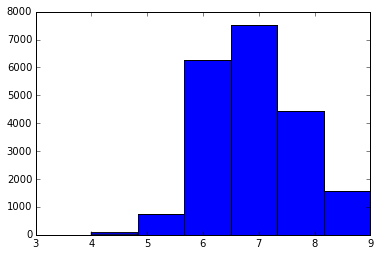
\includegraphics[height=3in]{reliability}
%\end{centering}
%\end{figure}

%While the focus of this paper has been to question the validity of SET as measures of teaching effectiveness, by showing that gender is a stronger predictor of SET scores than student performance, the academic research on SET suggests that reliability may also be an issue. Using the data from Sciences Po, we check for the reliability of students' answers. 







\section{Conclusions}

%Implicit in the use of SET as a Push back on the notion of ``teaching effectiveness.''
%There ought to be \emph{some} interaction between characteristics of the
%instructor and those of the student.
%If ``effectiveness'' is intrinsic to the instructor, ratings in one class shouldn't depend on
%which other classes a student takes.
%Looking at ratings ``per student'' doesn't make sense if you are trying to
%measure some underlying platonic ``effectiveness'' intrinsic to the instructor.
%In particular,  a showing that individual students who give a particular instructor higher ratings
%get higher grades, does not point to ....\todo{fix me}

Teaching effectiveness is hard to define, even among higher-education researchers. 
There is a consensus that teaching effectiveness is multidimensional (e.g. \citep{Marsh1997}), and that universities must find incentives to encourage better teaching. 

We used nonparametric permutation tests to examine data collected  
\citet{Boring2015} and \citet{MacNell2014}, both of which find that gender biases prevent 
SET from objectively measuring teaching effectiveness. 
Our tests confirm that SET are more tightly related to 
instructor's perceived gender and to grade expectations than they are to learning, 
as measured by performance on the final exam. 
Instructors appear to be rated on a characteristic that is neither relevant nor in their control---their
gender--rather than on their ability to promote student learning. 
The extent and direction of gender biases depend on context, making it
impossible to adjust for such biases to ``level the playing field.'' 
While the French university data show a positive male student bias for male instructors, 
the experimental US setting suggests a positive female student bias for male instructors.
And the biases in the French university setting vary by discipline.
We would also expect the bias to depend on class size, format, level, and a host of other variables.

Instead of measuring teaching effectiveness, SET appear to be a measure of student satisfaction \citep{StarkFreishtat2014}. 
Students may be satisfied or dissatisfied with courses for reasons outside of the control of instructors,
such as instructor gender. 
None of this is to say that there is \emph{no} connection between SET and student
performance: the correlation can be positive or negative, depends on context, and generally
is not statistically significant.
While student satisfaction may contribute to teaching effectiveness, it is not teaching effectiveness,
and our results show that SET are better measures of student grade expectations and of instructor 
gender than they are of teaching effectiveness.    

Gender and expected grades are not the only variables unrelated to teaching effectiveness that other studies have shown predict SET \citep{ADD_CITATIONS}.
Given the many variables that are likely to bias SET scores and whose weight in SET are likely to change from one learning environment to another, it would be impossible to control for all these variables to make SET a valid measure of teaching effectiveness. Furthermore, the direction of biases appear to be context dependent. 

Among the instructor characteristics alongside gender, race has also been shown to be correlated with SET scores.  In studies conducted in the US, instructors of color appear to suffer from student biases similar to those that female instructors suffer from in our analysis. Minority instructors tend to receive significantly lower SET scores compared to white (male) instructors (e.g. \citet{Merritt2008}).\footnote{French law does not allow for the use of race-related variables in data sets. We were thus unable to test for potential racial biases in SET scores in the context of our French university.} Other instructor-related characteristics likely to be unrelated to teaching effectiveness have been shown to be predictors of SET scores, such as age \citep{Arbuckle2003}, charisma \citep{Shevlin2000} and physical attractiveness (e.g. \citet{Riniolo2006} and \citet{Hamermesh2005}).  

Other factors still unrelated to factors that an instructor can control may be related to SET scores.  
Variables related to the teaching environment, class time, class size, mathematical content of the course, etc. may matter. 
For instance, \citet{Hill2010} show that students' perceptions of classroom environment factors (such as seating characteristics or lighting) have an impact on student ratings of instructors. 
They find that differences in the physical characteristics of classrooms influence students' overall satisfaction with a course, and have an impact on student evaluations of criteria such as their perceptions of how organized their instructors are.

Hundreds of studies discuss and question the validity of SET as a measure of teaching effectiveness 
(see \citet{Pounder2007} for a review). 
Some studies find results that are similar to ours, with male students expressing biases in favor of male instructors (e.g. \citet{Basow1987}; \citet{Kaschak1978}). 
Other studies find that the gender and SET is uncorrelated or that the relationship is weak (e.g. \citet{Bennett1982}; \citet{Centra2000}; \citet{Elmore1974}). 
While some studies tend to suggest that SET are not a valid measure of teaching effectiveness (e.g. \citet{Galbraith2012} and \citet{Carrell2010a}), others argue that SET are valid and reliable measures of teaching effectiveness (e.g. \citet{Benton2012} and \citet{Centra1977}). 
While there is no consensus among academics on the issue of validity, the fact that different 
studies show such a wide variety of results suggests that validity varies with contexts. 
This fact, in itself, shows that SET are not universally valid and should be used by universities with great caution.  

In the US, SET have two primary uses: 
to help instructors improve their teaching and to help the administration make personnel decisions, such as
hiring or promoting instructors. 
We recommend discontinuing the second use of SET, given the strong student biases that 
influence SET, even on ``objective'' items. 
In fact, in France, the French Ministry of Higher Education and Research upheld in 2009 a 1997 decision of the French State Council that public universities can use SET only to help tenured instructors improve their pedagogy, and that the administration may not  use SET in decisions that might affect 
tenured instructors' careers (cf. \citet{Boring2015ofce}). 

Our results suggest that the existence of gender biases in SET is context dependent. 
To test for the external validity of our results, we encourage the replication of our analysis in different settings. The results we find suggest that, in some contexts, female instructors may receive lower than average SET scores, despite being as effective instructors as men, only because of student biases in favor of male instructors. The use of SET therefore unfairly penalizes women, and can have large consequences on their academic careers. Our results more generally emphasize that, at least in some contexts, instructors are being unfairly judged based on variables that are out of their control, potentially leading to negative consequences on their careers in academia. We encourage universities to study potential biases that may occur in their contexts, and to take appropriate measures so as to not penalize instructors for variables that are out of their control.
 

\bibliographystyle{abbrvnat}
\bibliography{SETs}

\end{document}

